\chapter{Présentation de Deltacad}
\section{Présentation génerale}
La société Deltacad, basée à Compiègne, est spécialisée, depuis plus de 20 ans, dans la conception, la réalisation, la maintenance et la diffusion d'applications scientifiques et techniques, ainsi que la réalisation d'études avancées s'appuyant sur l'utilisation des logiciels développés.
Les clients de Deltacad sont majoritairement des grands groupes industriels ou des collectivités/institutionnels répartis dans 4 grands secteurs équilibrés :
\begin{itemize}
\item Environnement: CEREMA, DREAL, EPLoire, EPAMA, BRGM, Vendée-Eau, 
Oise-Aisne.
\item Energie et génie civil: AREVA, CEA, CERN, EDF, ENGIE, GRTGaz, EGIS,
Vallourec, Fondation Louis Vuitton, Setra, Vinci, TRACTEBEL, ...
\item Aéronautique, ferroviaire et naval: AIRBUS,
COMAC, DAPA, Dassault Aviation, MBDA, SAFRAN, STELIA, ...; ALSTOM,
SNCF ; AGCO (Challenger, Fendt, ...) ; Caterpillar, Volvo, ...
\item Automobile: Constructeurs automobile (PSA, BMW, ...) ; équipementiers 
(SOGEFI, Saint Gobain, Valéo, Delphi, ...) ; Sidérurgie (ArcelorMittal, Corus, Nippon Steel, ...) 
\end{itemize}
Deltacad noue également de forts partenariats avec des équipes universitaires : UTC dans le cadre du laboratoire commun DIMEXP, UTBM, UTT, ECN, ENSAM, INSA, dans le cadre de projets R\&D. 
Les équipes de Deltacad sont ainsi régulièrement enrichies des compétences de stagiaires et d'alternants des différentes universités partenaires, pour mener à bien des projets à fort potentiel d'innovation.

\newpage
\section{Les produits}
Deltacad assure le développement et le support de différents logiciels :
\begin{itemize}
\item \textbf{Gamme DeltaMESH} : DeltaMESH est dédiée à la modélisation géométrique et au maillage de modèles surfaciques issus des logiciels de \gls{CAO}. (“Nos produits – Deltacad.fr”) Le maillage consiste à transformer un modèle CAO en un objet tridimensionnel composé de polygones exploitable pour des applications de visualisation et/ou de simulation. Le logiciel autorise des maillages automatiques directement sur des modèles CAO en supprimant l’étape 
fastidieuse de nettoyage de ces modèles. DeltaMESH se décline en plusieurs 
produits, chacun répondant à un besoin particulier : DeltaMESH Stamping dédié 
à la simulation des process de fabrication (emboutissage, fonderie ...), 
DeltaMESH Fillet, outil de rayonnage automatique de maillages possédant des 
arêtes vives, DeltaMESH FEM, un mailleur permettant de générer des maillages 
de qualité "éléments finis" destinés à différents types de calculs (mécanique, thermique...).
\begin{figure}[H]
    \centering
    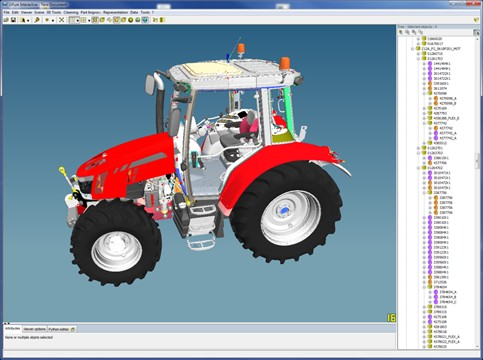
\includegraphics[height=8cm]{ressources/images/DeltaMesh.jpg}
    \caption{DeltaMesh}
\end{figure}

\item \textbf{Osiris-inondations et Osiris-Multirisques} : Osiris-inondations est un outil d'aide à la réalisation de Plans Communaux de Sauvegarde (PCS) destinés aux élus locaux. Ses fonctionnalités vont de la simulation de la montée des eaux, à la gestion d'une situation de crise en cas d'inondation et jusqu'à la réalisation de plans d'interventions pour les communes touchées. Osiris-Multirisques étend ces possibilités aux risques naturels et technologiques.

\begin{figure}[H]
    \centering
    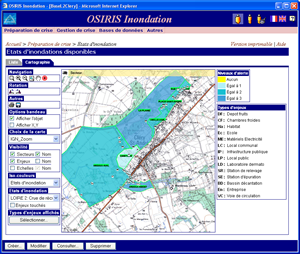
\includegraphics[height=8cm]{ressources/images/osiris-inondations.png}
    \caption{Osiris-inondations}
\end{figure}

\item \textbf{Code\_Aster} : Code\_Aster est un logiciel de simulation par éléments finis développé et utilisé par EDF pour ses études en mécanique des structures. Deltacad assure son développement et le support pour les utilisateurs de EDF.

\begin{figure}[H]
    \centering
    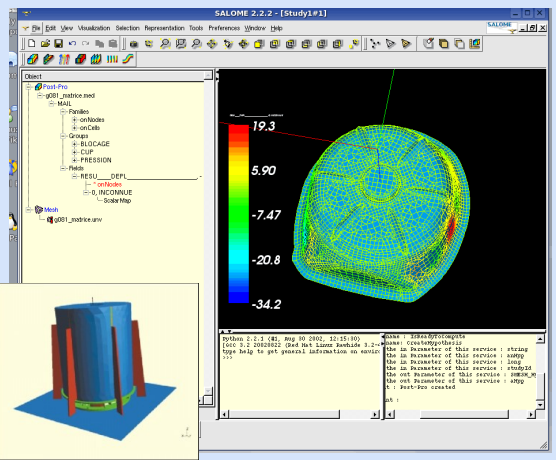
\includegraphics[height=8cm]{ressources/images/Code_Aster.png}
    \caption{Code\_Aster}
\end{figure}

\end{itemize}

\newpage
\section{Les services}
Outre les produits mentionnés ci-dessus, Deltacad offre également différents services à ses clients, notamment les suivants :
\begin{enumerate}
\item \textbf{Expertise et conseil en systèmes d'information scientifiques et techniques d'entreprise}\\ Deltacad apporte ici toute son expertise pour répondre à des questions stratégiques d'évolutions de logiciels ou d'organisation que se posent ses clients. Ces questions recouvrent des aspects variés :  
\begin{itemize}
\item Audits de logiciels (architecture, évolutivité, portabilité, performances...)
\item Choix de composants logiciels stratégiques
\item Validation externe de logiciel de simulation (taux de couverture, robustesse, qualité des résultats...)
\item Plan Qualité logiciel
\item Choix et méthodologie d'utilisation des logiciels
\item Capitalisation du savoir-faire métier
\item Rédaction de cahier des charges logiciels
\end{itemize}
\item \textbf{Développement d'applications scientifiques et techniques} \\
De par son expérience des différents métiers et techniques, Deltacad développe des logiciels solutions permettant de répondre aux besoins spécifiques de ses clients. Deltacad maîtrise, en partenariat avec son client, la réalisation complète de l'application de sa conception à sa maintenance.\\

Ce type de projet fait intervenir les différentes compétences de Deltacad pour mettre en exploitation chez le client la solution qui répondra aux besoins exprimés dans le cahier des charges. Les logiciels réalisés intègrent tout ou partie des fonctions suivantes :
\begin{itemize}
\item Interface utilisateur, visualisation 2D et 3D
\item Modélisation géométrique
\item Discrétisation, maillage
\item Modélisation de phénomènes physiques
\item Analyse de résultats
\item Gestion interne des données
\item Echange de données avec les systèmes extérieur
\end{itemize}
Ces logiciels solutions peuvent également intégrer certains composants de la librairie DeltaMESH Toolkit de Deltacad et/ou des outils du domaine public (Open Source).

\item \textbf{Intégration et couplage de logiciels (application métier)}\\ 
A partir des exigences métier du client, Deltacad automatise le fonctionnement d'un ensemble de logiciels techniques pour réaliser une chaîne numérique compléte, composée par exemple de :
\begin{itemize}
\item Interfaces d'échanges de données avec les systèmes exitants du clients
\item Logiciels du marché
\item Logiciels métiers de l'entreprise cliente
\item Logiciels développés par Deltacad
\end{itemize}
Pour des environnements d'exploitation complexes (multi-sites, sécurité, gestion de charge ...), ces besoins sont satisfaits de manière optimale, par l'utilisation des technologies distribuées et Internet :
\begin{itemize}
\item Exploitation des spécificités de chaque machine
\item Répartition des tâches de traitement
\item Limitation des opérations de portage
\item Déploiement/Mise à jour facilités
\item Centralisation/Synchronisation des données et objets métiers
\item Contrôle d'accès aux données et aux applications
\end{itemize}
\item \textbf{Industrialisation et gestion déléguée de logiciels (TMA et MCO)}\\ 
Les entreprises clientes de Deltacad réalisent en interne des applications représentant un savoir-faire stratégique pour leurs métiers.

Tôt ou tard, il est nécessaire de les faire évoluer pour prendre en compte des besoins nouveaux ou des évolutions de l'environnement informatique. Bien souvent, les compétences et les moyens humains manquent alors à l'appel en raison de mobilité ou de réorganisation des entreprises, d'où un risque important de perte de savoir-faire.

C'est pourquoi Deltacad a développé les méthodes et l'organisation nécessaires pour intervenir sur tout ou partie du cycle de vie des logiciels métiers. Ceci garantit une continuité de l'évolution et du support de l'application avec une totale visibilité pour l'entreprise cliente, tout en lui  permettant de se concentrer sur son métier.

Deltacad met ainsi à la disposition de ses clients des moyens analogues à ceux qui contribuent au succès de ses produits.

Outre la conception et le développement, les actions suivantes concourent à cette activité :
\begin{itemize}
\item Expertise/Analyse de l'existant
\item Reconception de tout ou partie des logiciels rentrant dans le cadre de la prestation
\item Amélioration des performances
\item Développement d'une interface utilisateur
\item Portage et migration sur de nouveaux environnement (UNIX, Windows NT, LINUX)
\item Documentation technique (manuels utilisateurs, docuementation informatique)
\item Validation des logiciels
\item Outils d'installation des logiciels
\item Packaging et documentation commerciale
\item Organisation des développements (multi-partenaires, multi-sites, multi-plateformes...)
\item Gestion de configuration et traçabilité
\item Support technique (hot-line, formation)
\item Maintenance (gestion des anomalies et des souhaits d'évolution, corrections des anomalies)
\item Diffusion au sein de l'entreprise ou auprès de clients externes
\end{itemize}
\item \textbf{Etudes et calculs de produits \& process}\\
La maîtrise de la simulation de nombreux phénomènes physiques (Mécanique, Thermique, Fluide) et la réactivité de Deltacad nous permettent de réaliser des simulations adaptées à différents contextes :
\begin{itemize}
\item Simulations à titre de validation de la conception
\item Simulation de type pré-dimensionnement pour orienter les choix de conception
\item Réalisation de plan d'expériences numériques
\item Modélisation de process de fabrication
\end{itemize}
Pour garantir la réactivité et la qualité des résultats, Deltacad dispose de moyens de calculs et de logiciels performants, et d'une expérience de plus d'une quinzaine d'années en modélisation.

Ces études peuvent également être réalisées avec des logiciels spécifiques développés par Deltacad pour les besoins particuliers de l'étude.
\end{enumerate}


\newpage
\section{L'équipe de travail}
Le stage que j'ai effectué avait pour objectif de développer le logiciel pour le sujet de recherche ETREL « inspEction auTomatique de défauts en temps Réel et en ligne à partir de données multi-sources et via l’usage de machines apprEnantes : 
contribution à L’industrie 4.0 », j’ai donc rejoint l’équipe qui travaille sur ce sujet de recherche, composée de deux ingénieurs : 
\begin{itemize}
\item Harvey ROWSON, chef de projet.
\item Julien MONVILLE, ingénieur de développement.
\end{itemize}
Dans le cadre de mon travail, notre équipe utilise le \textbf{WebEX} pour la communication et la planification des tâches, et \textbf{SmartSVN} pour la gestion des versions des logiciels.
